\chapter{Introduction}
\section{What is \Kieker?}

The \Kieker{} framework allows to monitor and to analyze the runtime behavior %
of Java applications. Examples of runtime behavior are application-internal %
control flows and response times of method executions. %
% Normal ({}``plain) Java applications can be arranged with the framework as well %
% as server based Java web applications. 
% The framework itself has been developed with regard to providing an easy manageable, %
% maintainable piece of software, which can be included uncomplicated into both, %
% new and existing software projects. 
Kieker has been designed for continuous operation, inducing only a very low %
overhead during the monitoring. 
% Kieker can probe whole method calls as well as single statements (e.g. a = a + 1).\\ 

% This is the component diagram of Kieker (the satellite).
\begin{figure}[H]\centering
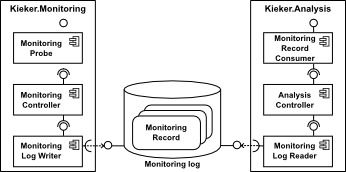
\includegraphics[width=0.73\textwidth]{images/kiekerComponentDiagram-woCloud-bw-w-record-newNames}
\caption{Overview of the framework components}
\label{Figure:KiekerComponentDiagram}
\end{figure}
		
\noindent Figure \ref{Figure:KiekerComponentDiagram} shows that the framework %
is structured into two main components:% \KiekerMonitoringPart{} and \KiekerAnalysisPart{}:
\begin{description}
 % Both items get notify-tags because of the important information in here.
\item[\KiekerMonitoringPart]
is responsible for the program instrumentation, data %
collection and logging.  Its core is the singleton class \class{MonitoringController} %
\notify which receives the monitoring data in so-called records and %
writes these records into the configured monitoring log which can, for example, %
be located in a filesystem or in a database.
\item[\KiekerAnalysisPart]
is responsible for the evalution and possible visualization of the %
recorded information. Its core is the class \class{AnalysisInstance} \notify %
which manages the lifecycle of the readers and all plugins which shoud analyze %
the stored information.
\end{description}


\noindent Both parts are composed of subcomponents which can just be used or %
replaced by customized implementations. The important interaction pattern among %
the components is illustrated in Figure \ref{Figure:KiekerCommunicationDiagram} %
but will be explained furthermore throughout the course of this tutorial. %

% This image shows the communication diagram of the different components.
\begin{figure}[H]\centering
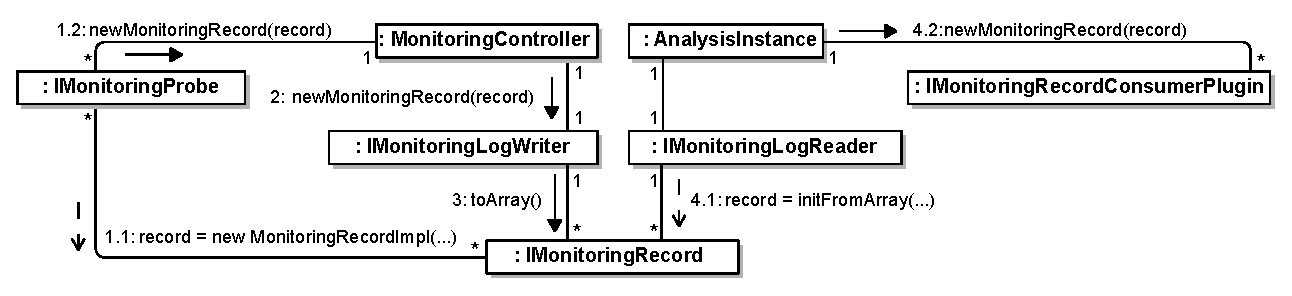
\includegraphics[width=1\textwidth]{images/kiekerCommunications-revisedReArranged-woMonitoringLog-bw-newNames}
\caption{Communication among \Kieker{} framework components}
\label{Figure:KiekerCommunicationDiagram}
\end{figure}
		
% Notify-tag because it is explained how Kieker works.
\noindent\notify The monitoring probes create the monitoring records and deliver %
them to the monitoring controller. The monitoring controller uses the monitoring %
log writers to persist the given records which can later be read by a monitoring %
log reader who creates a monitoring record again. These records can then be used %
by the consumers in nearly every way.

\section{Features}
\TODO{The features-part has yet to be filled.}
	
\section{The purpose of this tutorial}
% Short explanation what the tutorial will show now.
This tutorial will take a closer look at both, the \KiekerMonitoringPart{}- and %
the \KiekerAnalysisPart-part. It will be described on the one hand how %
\KiekerMonitoringPart{}  can be used to instrument Java programs %
with \Kieker\ and to let them execute under monitoring, so that the recorded %
information can be persisted and on the other hand \KiekerAnalysisPart{} %
will be used for processing the recorded data.

Before this tutorial goes deeper into the single parts of the framework, it %
shows how to create and execute a simple example.
